\chapter{Evaluation and Analysis}

In the previous chapter, a few approaches that could improve the genetic solver were presented.
The best results give a combination of the genetic solver with added probabilities and parameter tuning.
Other methods like an adaptive crossover rate or population without duplicated individuals give less effect on the results.

On the other hand, we get valid results only for one problem. What if the problem will be smaller or bigger?
The evaluation was done to find out how all approaches work with different problem sizes. 

\section{Evaluation}

To evaluate genetic solver, a benchmark set of 36 problems was used.
Each problem with different parameters that describes them.
All parameters are:

\begin{itemize}
	\item variant - [2, 4] ,
	\item request - [1, 2, 4],
	\item depth - [2, 3, 4],
	\item resources - [50, 100].
\end{itemize}

This set was tested with several versions of genetic solver:

\begin{itemize}
	\item basic,
	\item basic with tuned parameters,
	\item with added parameters,
	\item with added parameters and tuning,
	\item with adaptive crossover rate,
	\item with adaptive crossover rate and tuning,
	\item without duplicates in a population,
	\item without duplicates in a population and tuning.
\end{itemize}

Each version of the genetic solver tries five times to solve each problem.

The benchmark set was run on the hardware set with Inlet 8th Generation \todo{complete}

Benchmark trying so solve each task, if a solution was valid, genetic solver start to solve next problem. If after five attempts the genetic solver did not find a valid solution, it proceeded to the next problem.

Figure~\ref{fig:EvaluationNumberOfSolvedProblems} shows the number of problems in which genetic solver get a valid result.
All previously presented approaches get more valid results in comparison to the basic version.

\begin{figure}
	\centering
	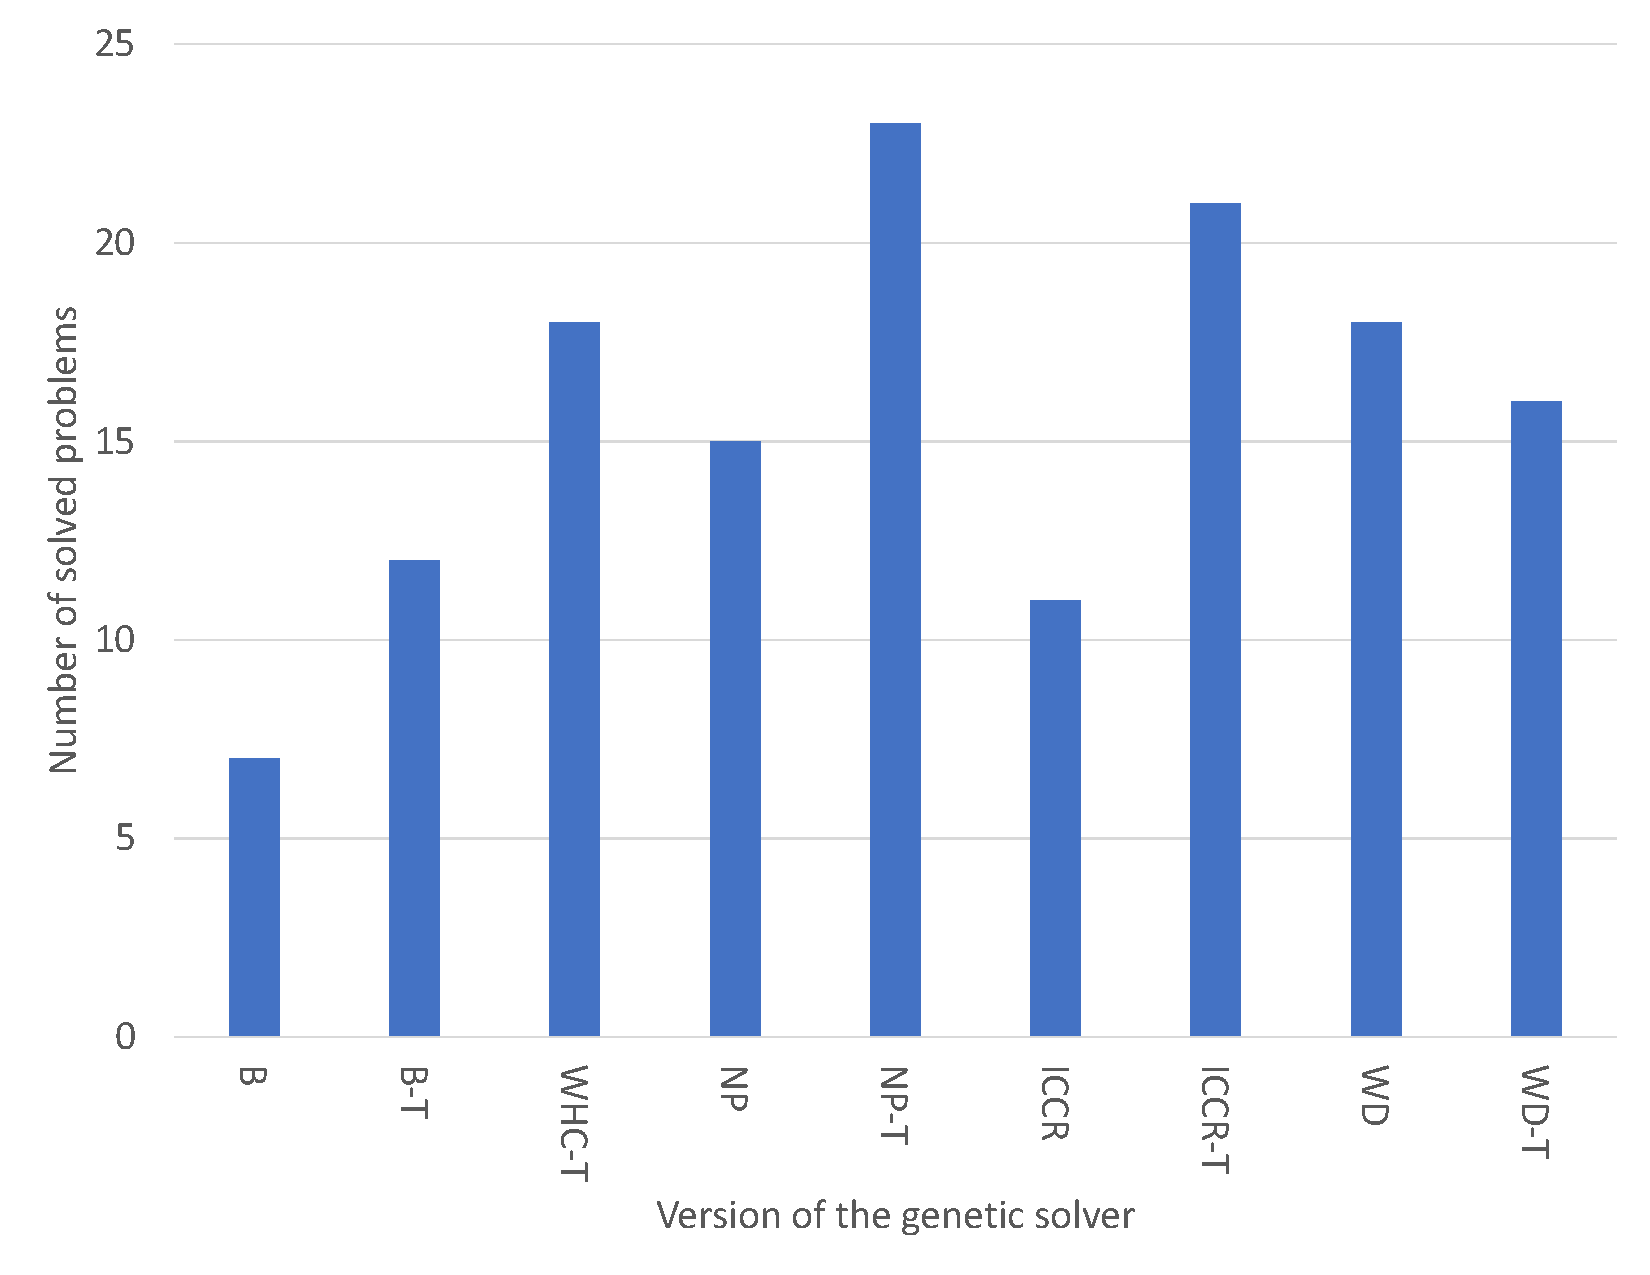
\includegraphics[width=\textwidth]{images/EvaluationNumberOfSolvedProblems.pdf}
	\caption[Number of problems for each version of the genetic solver]{Number of solved problems for each version of the genetic solver}
	\label{fig:EvaluationNumberOfSolvedProblems}
\end{figure}

\todo{when benchmark will be finished I will add more}

But what about energy?


Table~\ref{tab:EnergyTable} shows the percentage deviation of the found solution from the optimum.
The conclusion from this table is that if solver finds out valid results it will be optimal or near-optimal.

\begin{table}
	\begin{tabularx}{\textwidth}{@{}rrrrr@{}}
		\toprule
		\textbf{Problem ID} & \textbf{Basic} &
		\textbf{with new probabilities} & \textbf{without duplicates in population} & \textbf{without duplicates in population + tuning} 
		\tabularnewline
		\midrule
		1 & 1.23 & 0.01 & 0 & 0
		\tabularnewline
		10 & 0.26 & 0.03 & 0 & 0
		\tabularnewline
		13 & 0.05 & 0.05 & 0.15 & 15.0
		\tabularnewline
		19 & 0.19 & 0.19 & 0 & 0
		\tabularnewline
		28 & 0.32 & 0 & 0.02 & 0
		\tabularnewline
		31 & 29.93 & 6.97 & 0.33 & 6.71
		\tabularnewline
		\bottomrule
	\end{tabularx}
	\caption{Table name}\label{tab:EnergyTable}
\end{table}

\begin{figure}
	\centering
	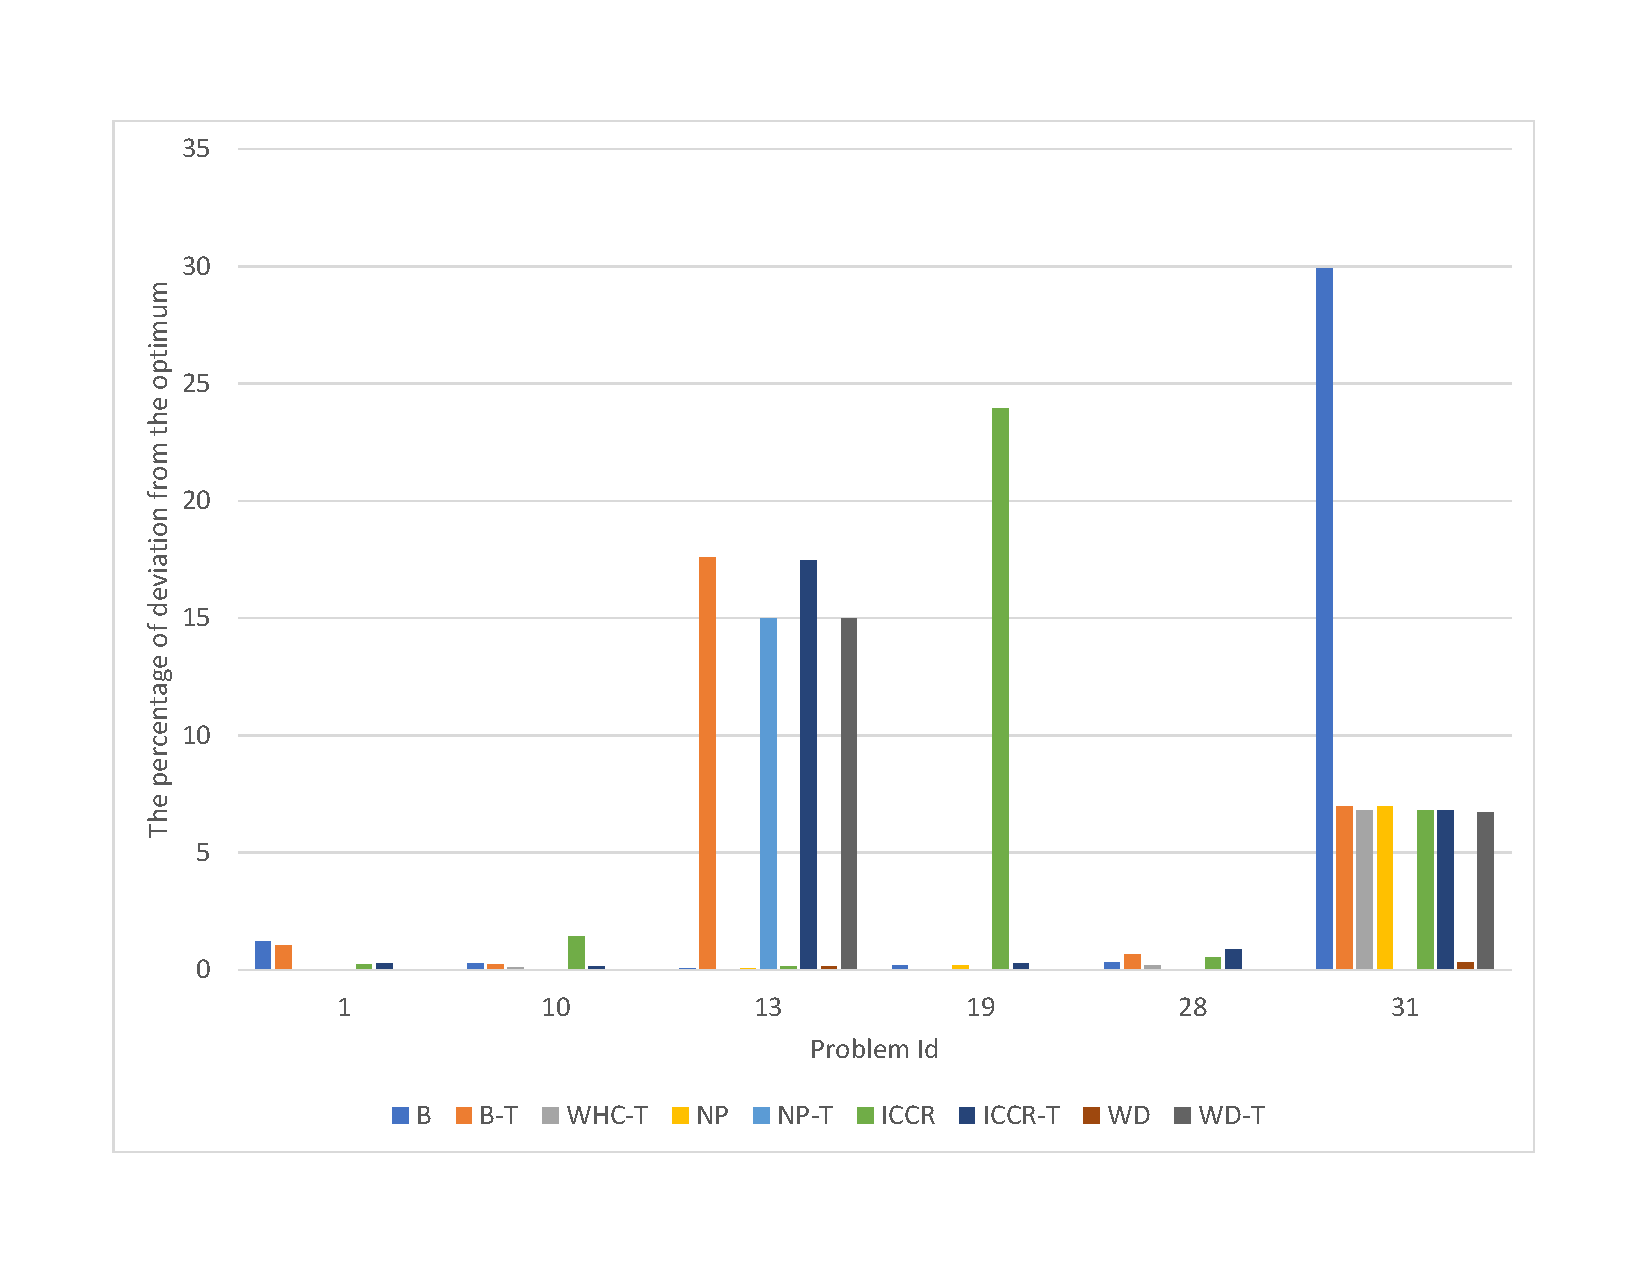
\includegraphics[width=\textwidth]{images/EnergyPercentage.pdf}
	\caption[]{}
	\label{fig:EnergyPercentage}
\end{figure}

The results also show that even with modifications, genetic solver could not get valid and optimal results for all problems.


\section{Analysis}

Benchmark showed that a genetic solver is not the best choice to solve the MquAT problem.
In this section, we presented an analysis of results, reasons why described in Chapter~\ref{chapter:Implementation} approaches, and optimizations have small efficiency.

A considerable influence on improving the performance of the genetic solver had several factors. Adding additional probabilities to the crossover and mutation operators, the crossover and mutation points began to change their position randomly.
Optimized parameters also improved results, but not in all cases.

But why did not all the improvements made give even more significant improvement, and why did the tuning of the parameters in several cases provide a worse result?

First, we optimized the parameters for a specific task, and, possibly, these optimized parameters are not optimal for other problems.
Second, the search space for parameters that have been optimized, more than 3 thousand configurations were measured and depicted in Figure~\ref{fig:SearchSpaceViewFull}.

\begin{figure}
	\centering
	\includegraphics[width=\textwidth]{images/SPEA2.pdf}
	\caption[]]{}
	\label{fig:SearchSpaceViewFull}
\end{figure}

There is not much useful information. Among the configurations, there are those that led to valid results (the number of contract violations is 0) and many that led to more contract violations.

\begin{figure}
	\centering
	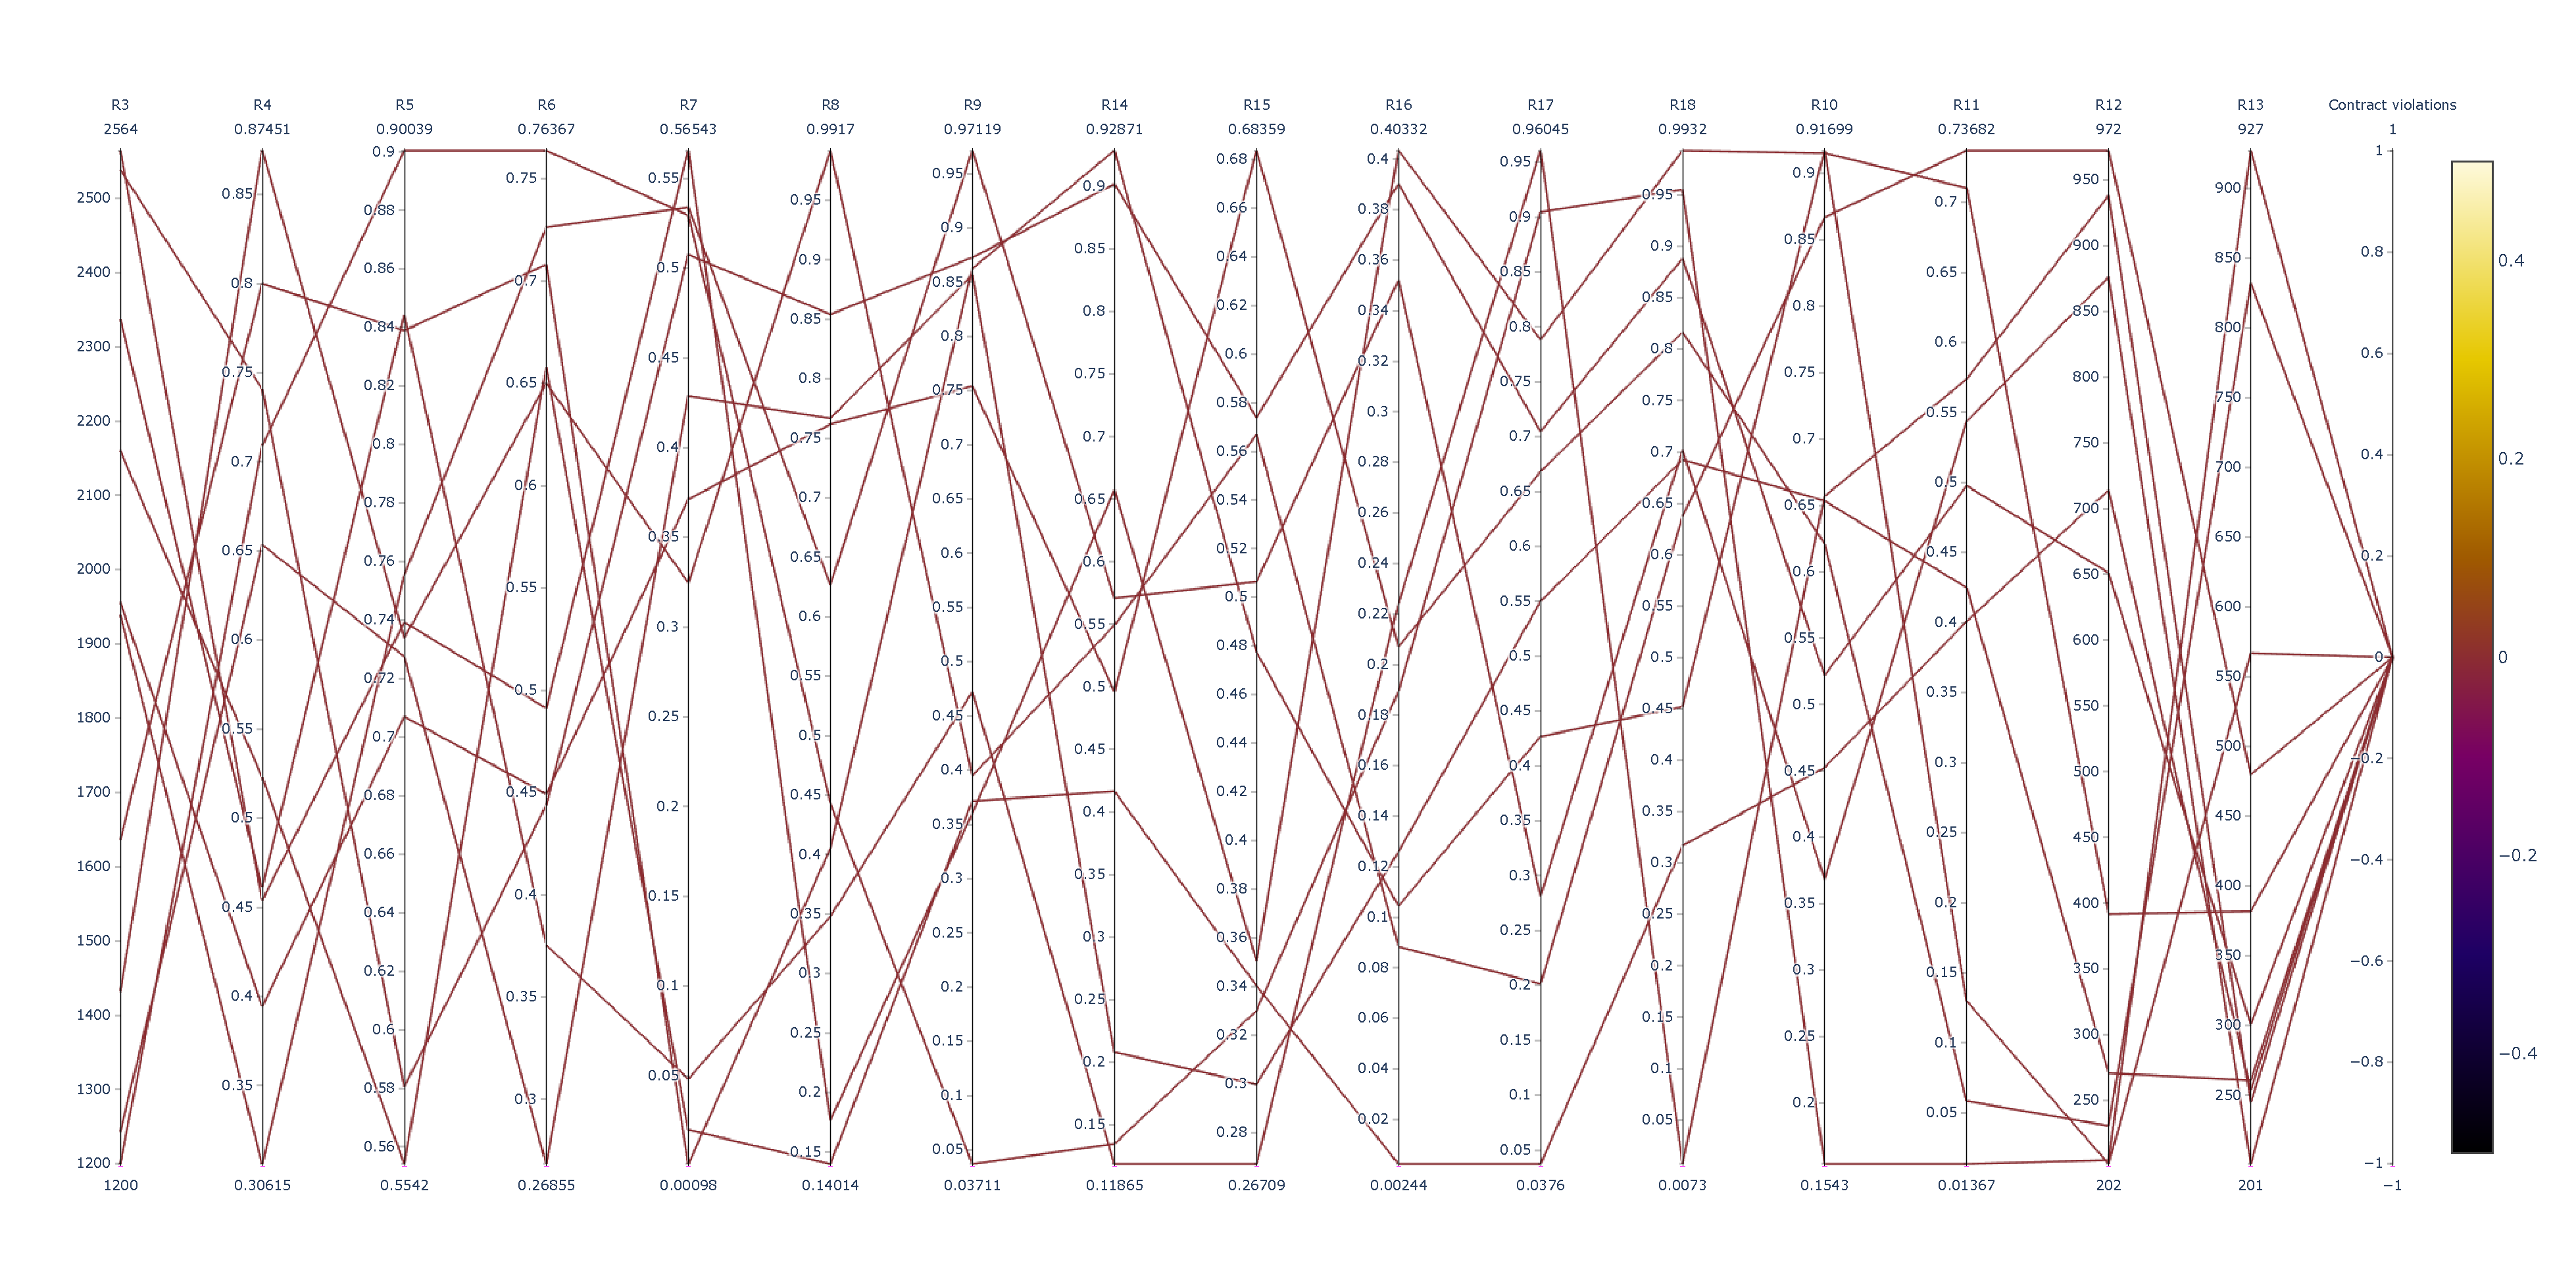
\includegraphics[width=\textwidth]{images/SPEA2_Zero_validity.html.pdf}
	\caption[]]{}
	\label{fig:SearchSpaceValid}
\end{figure}

Filtering out only those configurations that gave valid results, we got the search space shown in Figure~\ref{fig:SearchSpaceValid}. From the Figure~\ref{fig:SearchSpaceValid} it follows that there are no apparent dependencies between the parameters and the number of contract violations, or between the parameters themselves.

\begin{figure}
	\centering
	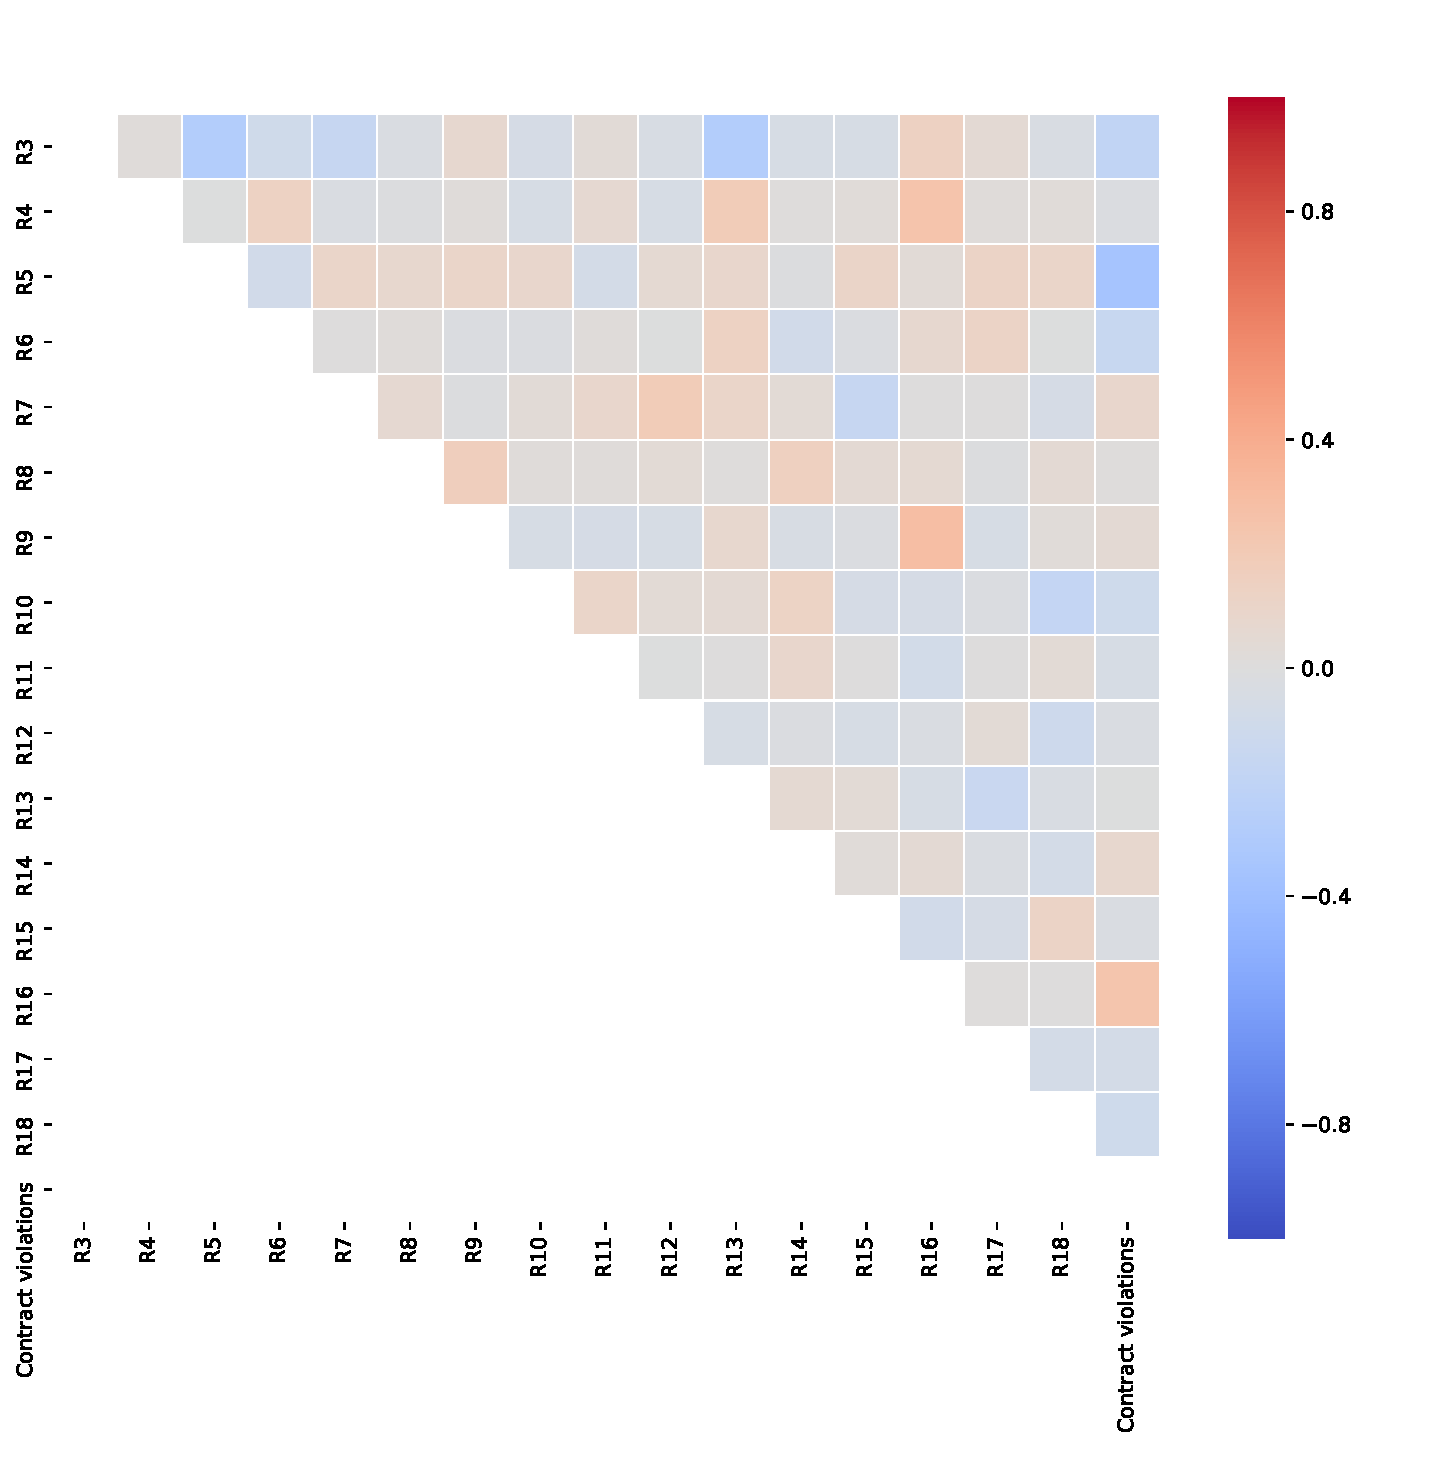
\includegraphics[width=\textwidth]{images/CorrelationAnalysis.pdf}
	\caption[]]{}
	\label{fig:CorrelationAnalysis}
\end{figure}

Cause Figure~\ref{fig:SearchSpaceViewFull} and Figure~\ref{fig:SearchSpaceValid} shows that search space view could not give any conclusions about dependencies between parameters or between parameters and number of contract violations, another method of analysis was performed.
We made a correlation analysis and it showed in Figure~\ref{fig:CorrelationAnalysis}. Colors indicate the level of correlation. Blue is the inverse correlation, that means that bigger value of parameter gives smaller number of contract violations. Red color means that bigger value o parameter gives bigger number of contract violations.
From the correlation analysis, we can conclude that there are no strong dependencies between the number of contract violations and parameters. There are two more important parameters: \texttt{CrossoverRate}(R5) and \texttt{CrossoverOnRandomRequestProbability}(R16).
Correlation analysis showed that the \texttt{CrossoverRate} need to has a big value. Also, conclusion from this analysis that small value  \texttt{CrossoverOnRandomRequestProbability}. It's also shows that we can remove this parameter. 

For further analysis of dependencies, graphs of the distribution of parameter pairs were constructed. Let us examine one representative distribution and, using another as an example, show how others look.

\begin{figure}
	\centering
	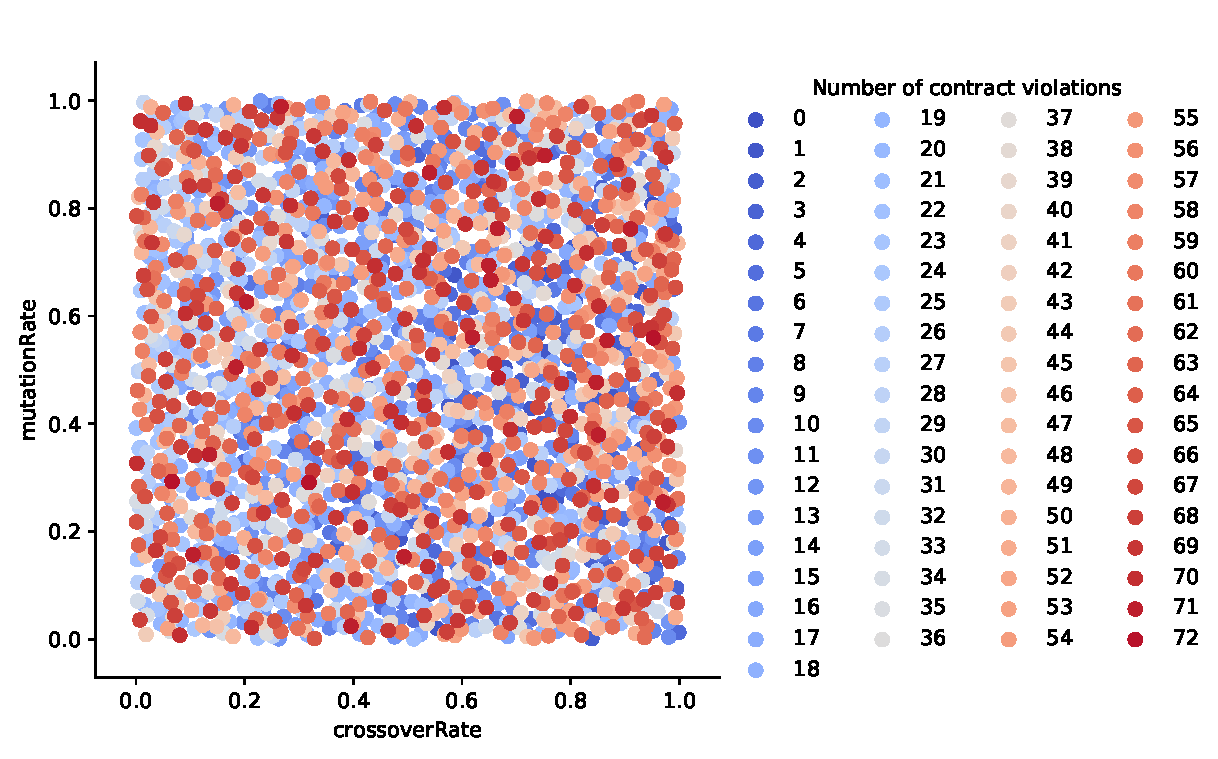
\includegraphics[width=\textwidth]{images/CrossoverRateVsutationRate.pdf}
	\caption[]]{}
	\label{fig:CrossoverRateVmutationRate}
\end{figure}

\begin{figure}
	\centering
	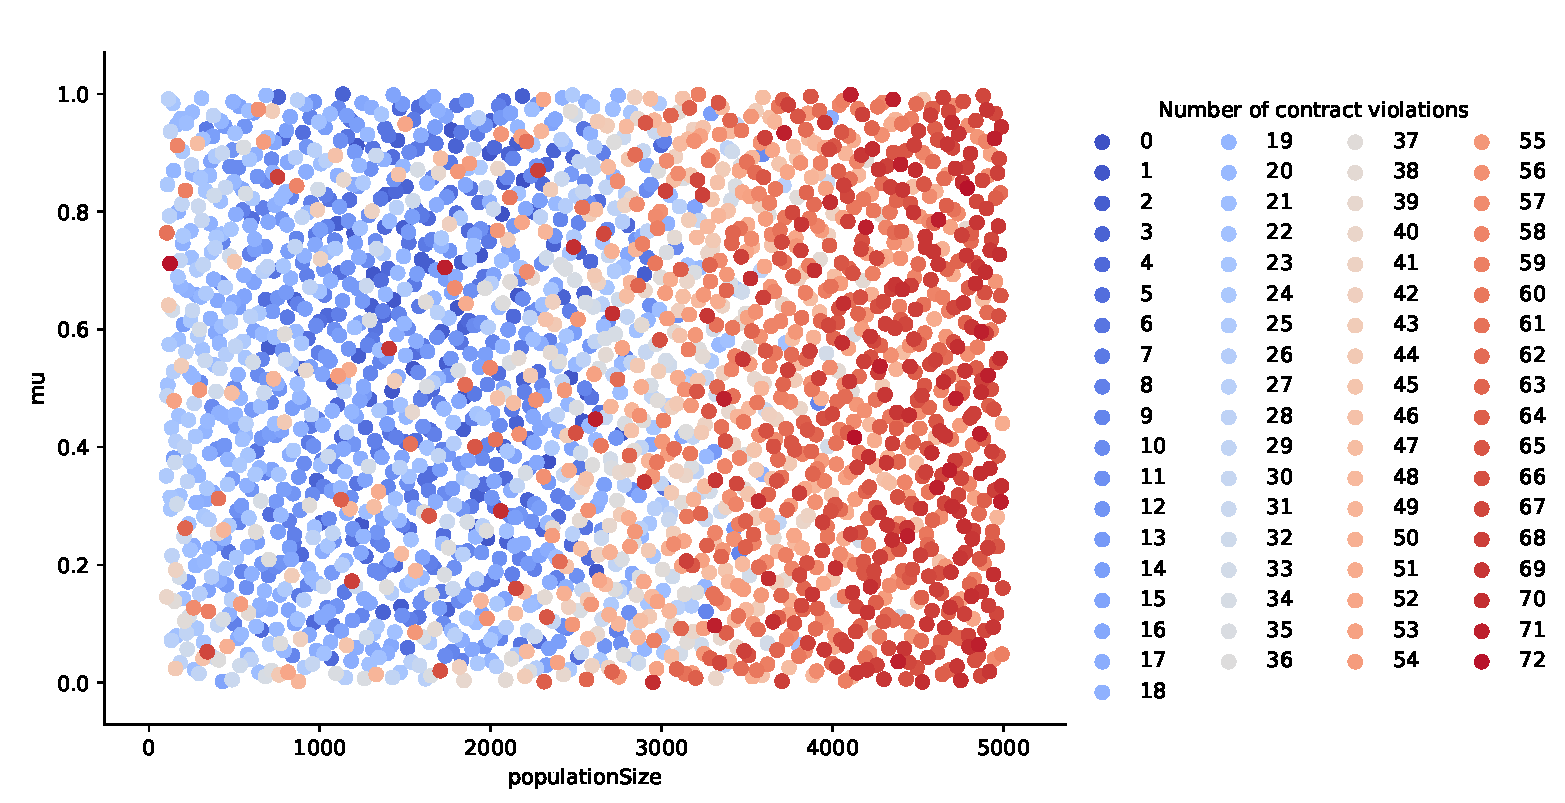
\includegraphics[width=\textwidth]{images/populatioSizeVsMu.pdf}
	\caption[]]{}
	\label{fig:populatioSizeVsMu}
\end{figure}

Any distribution associated with the population size parameter has a different look and shows that this parameter has an effect on the result.
Figure~\ref{fig:populatioSizeVsMu} shows an example of such distribution, and it is clearly seen that valid results, or close to valid, are in the range from 1000 to 2600.

At the same time, most distributions are similar to Figure~\ref{fig:CrossoverRateVsutationRate}, which shows the distribution of parameters of crossover rate and mutation rate. 
The Figure~\ref{fig:CrossoverRateVmutationRate} shows that valid, or close to valid results exist for all values of described parameters. That also confirms idea described in correlation analysis to remove some parameters like \texttt{CrossoverOnRandomRequestProbability} from the tuning and set it in the solver as 0.

\begin{figure}
	\subfloat[Name A]{%
		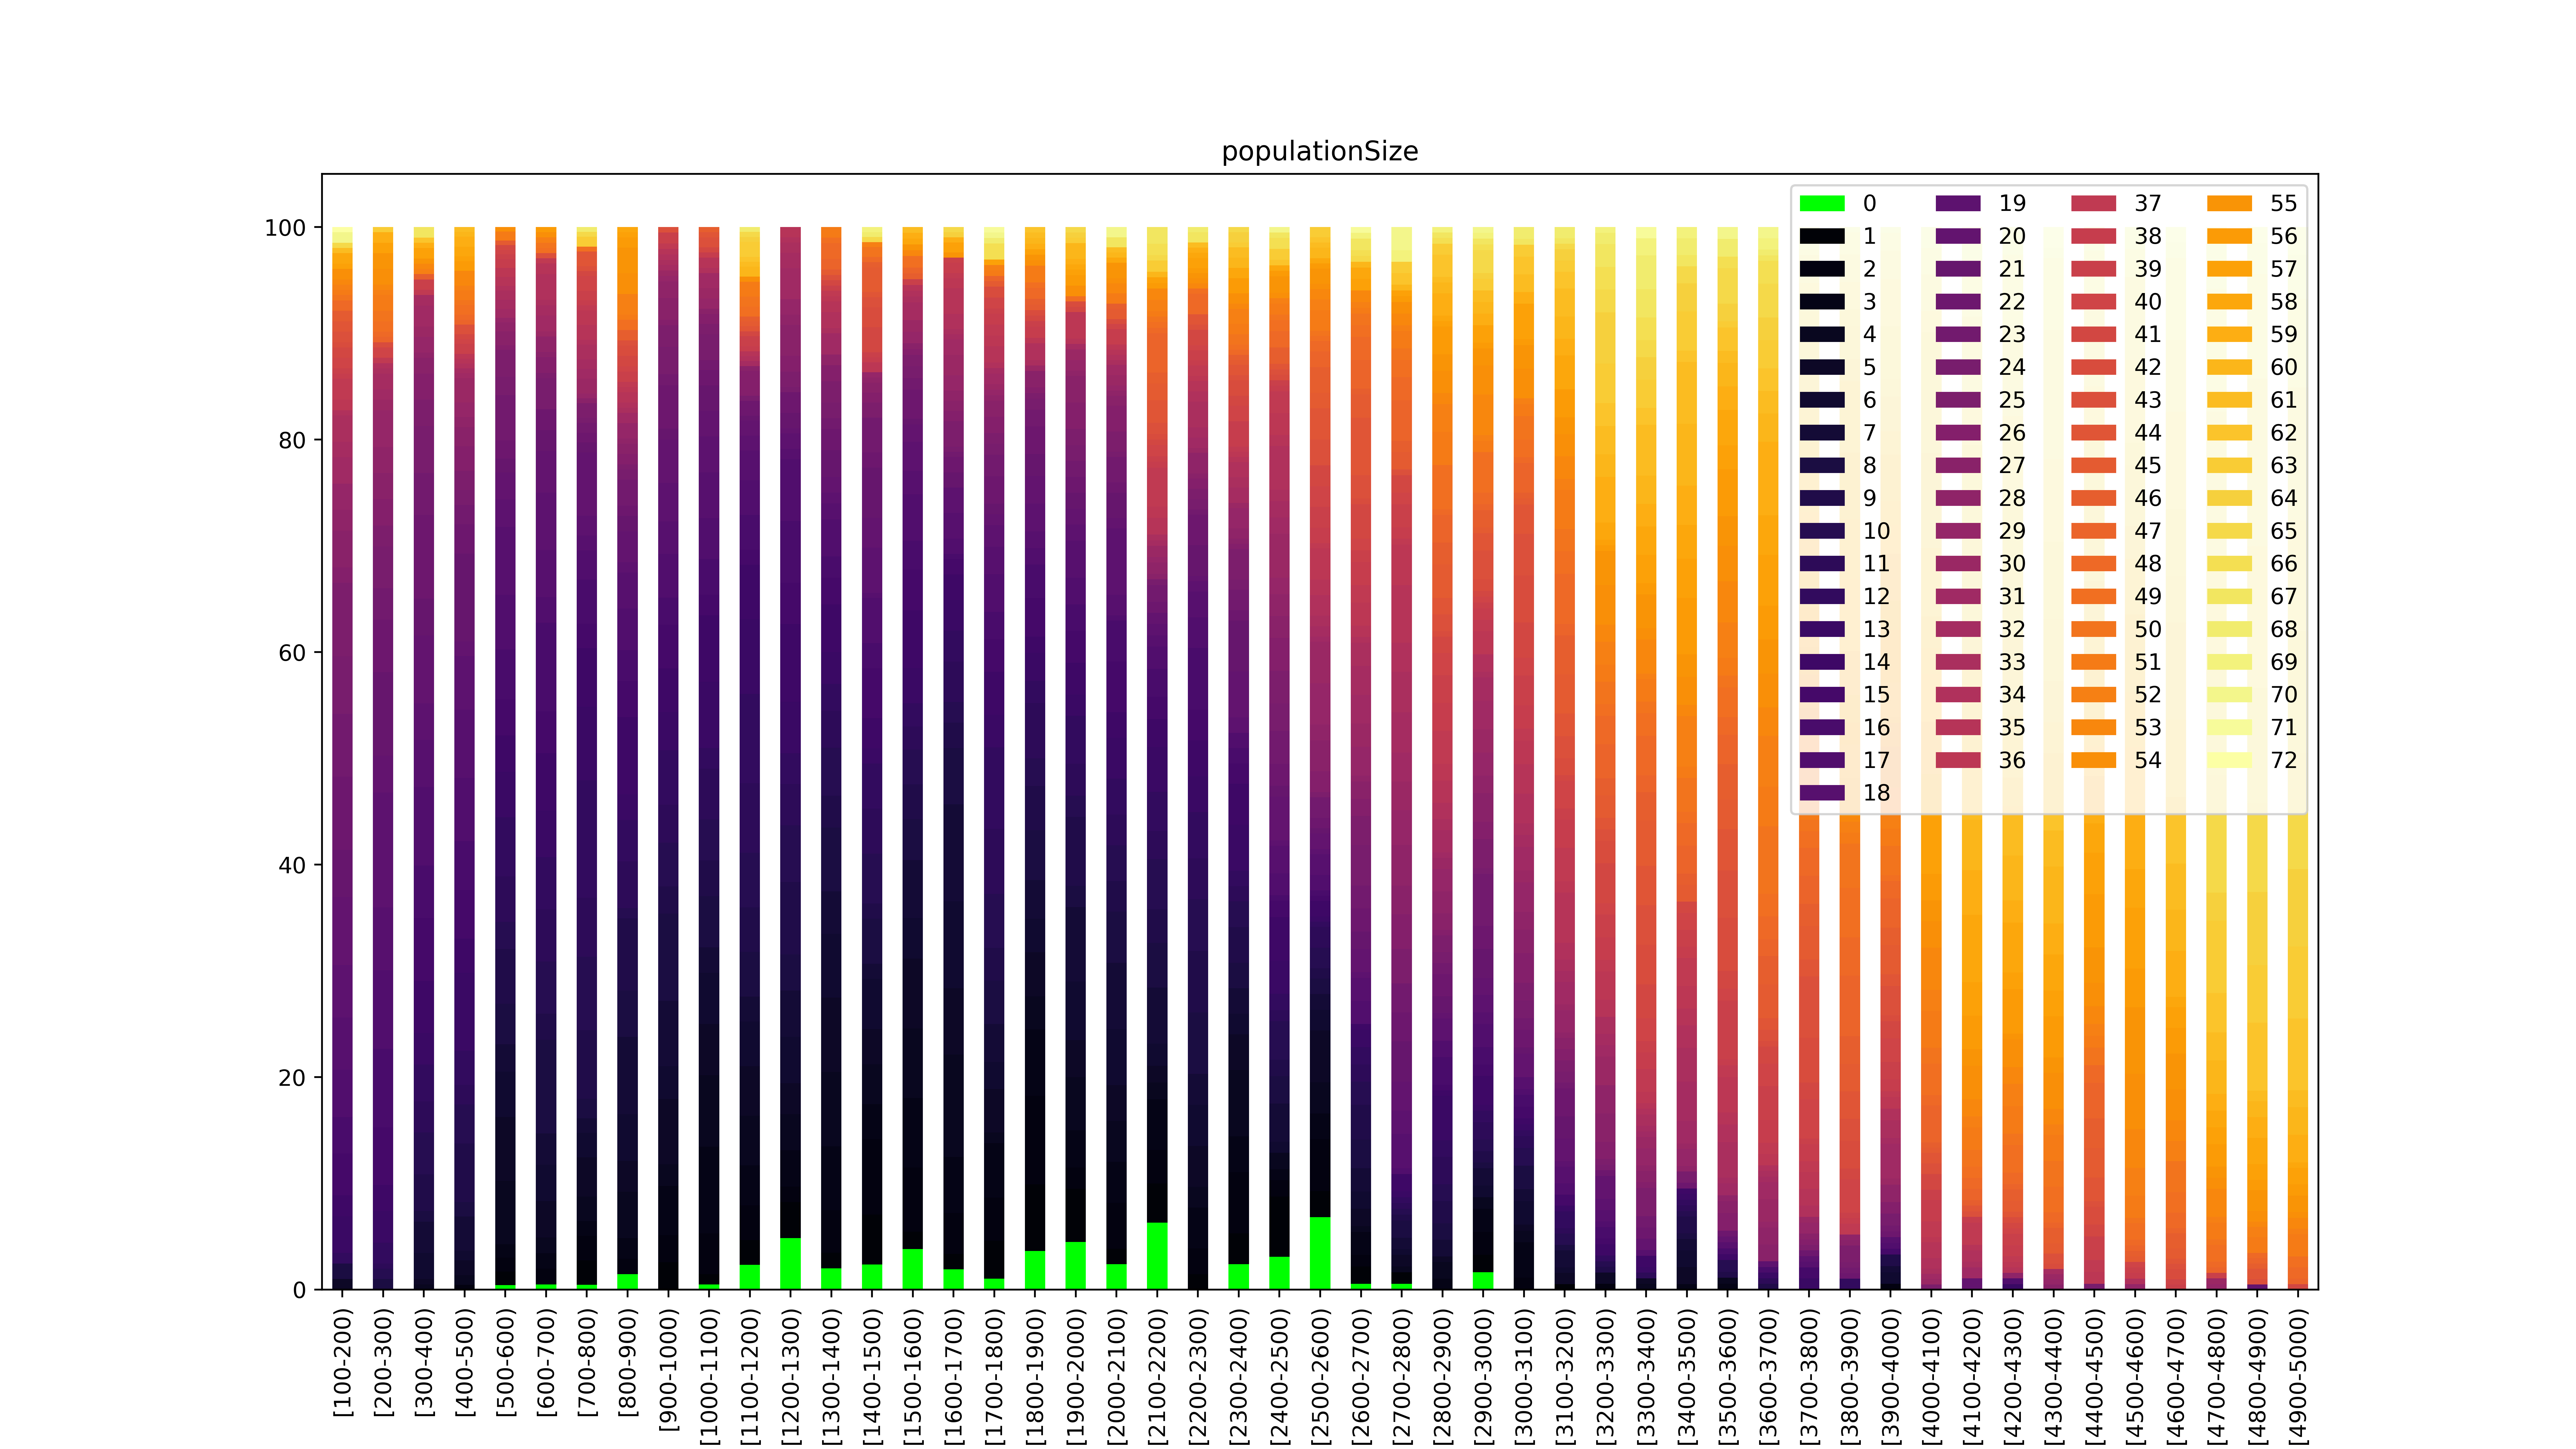
\includegraphics[clip,width=\textwidth]{images/populationSize_gradientBig.png}%
	}
	
	\subfloat[Name b]{%
		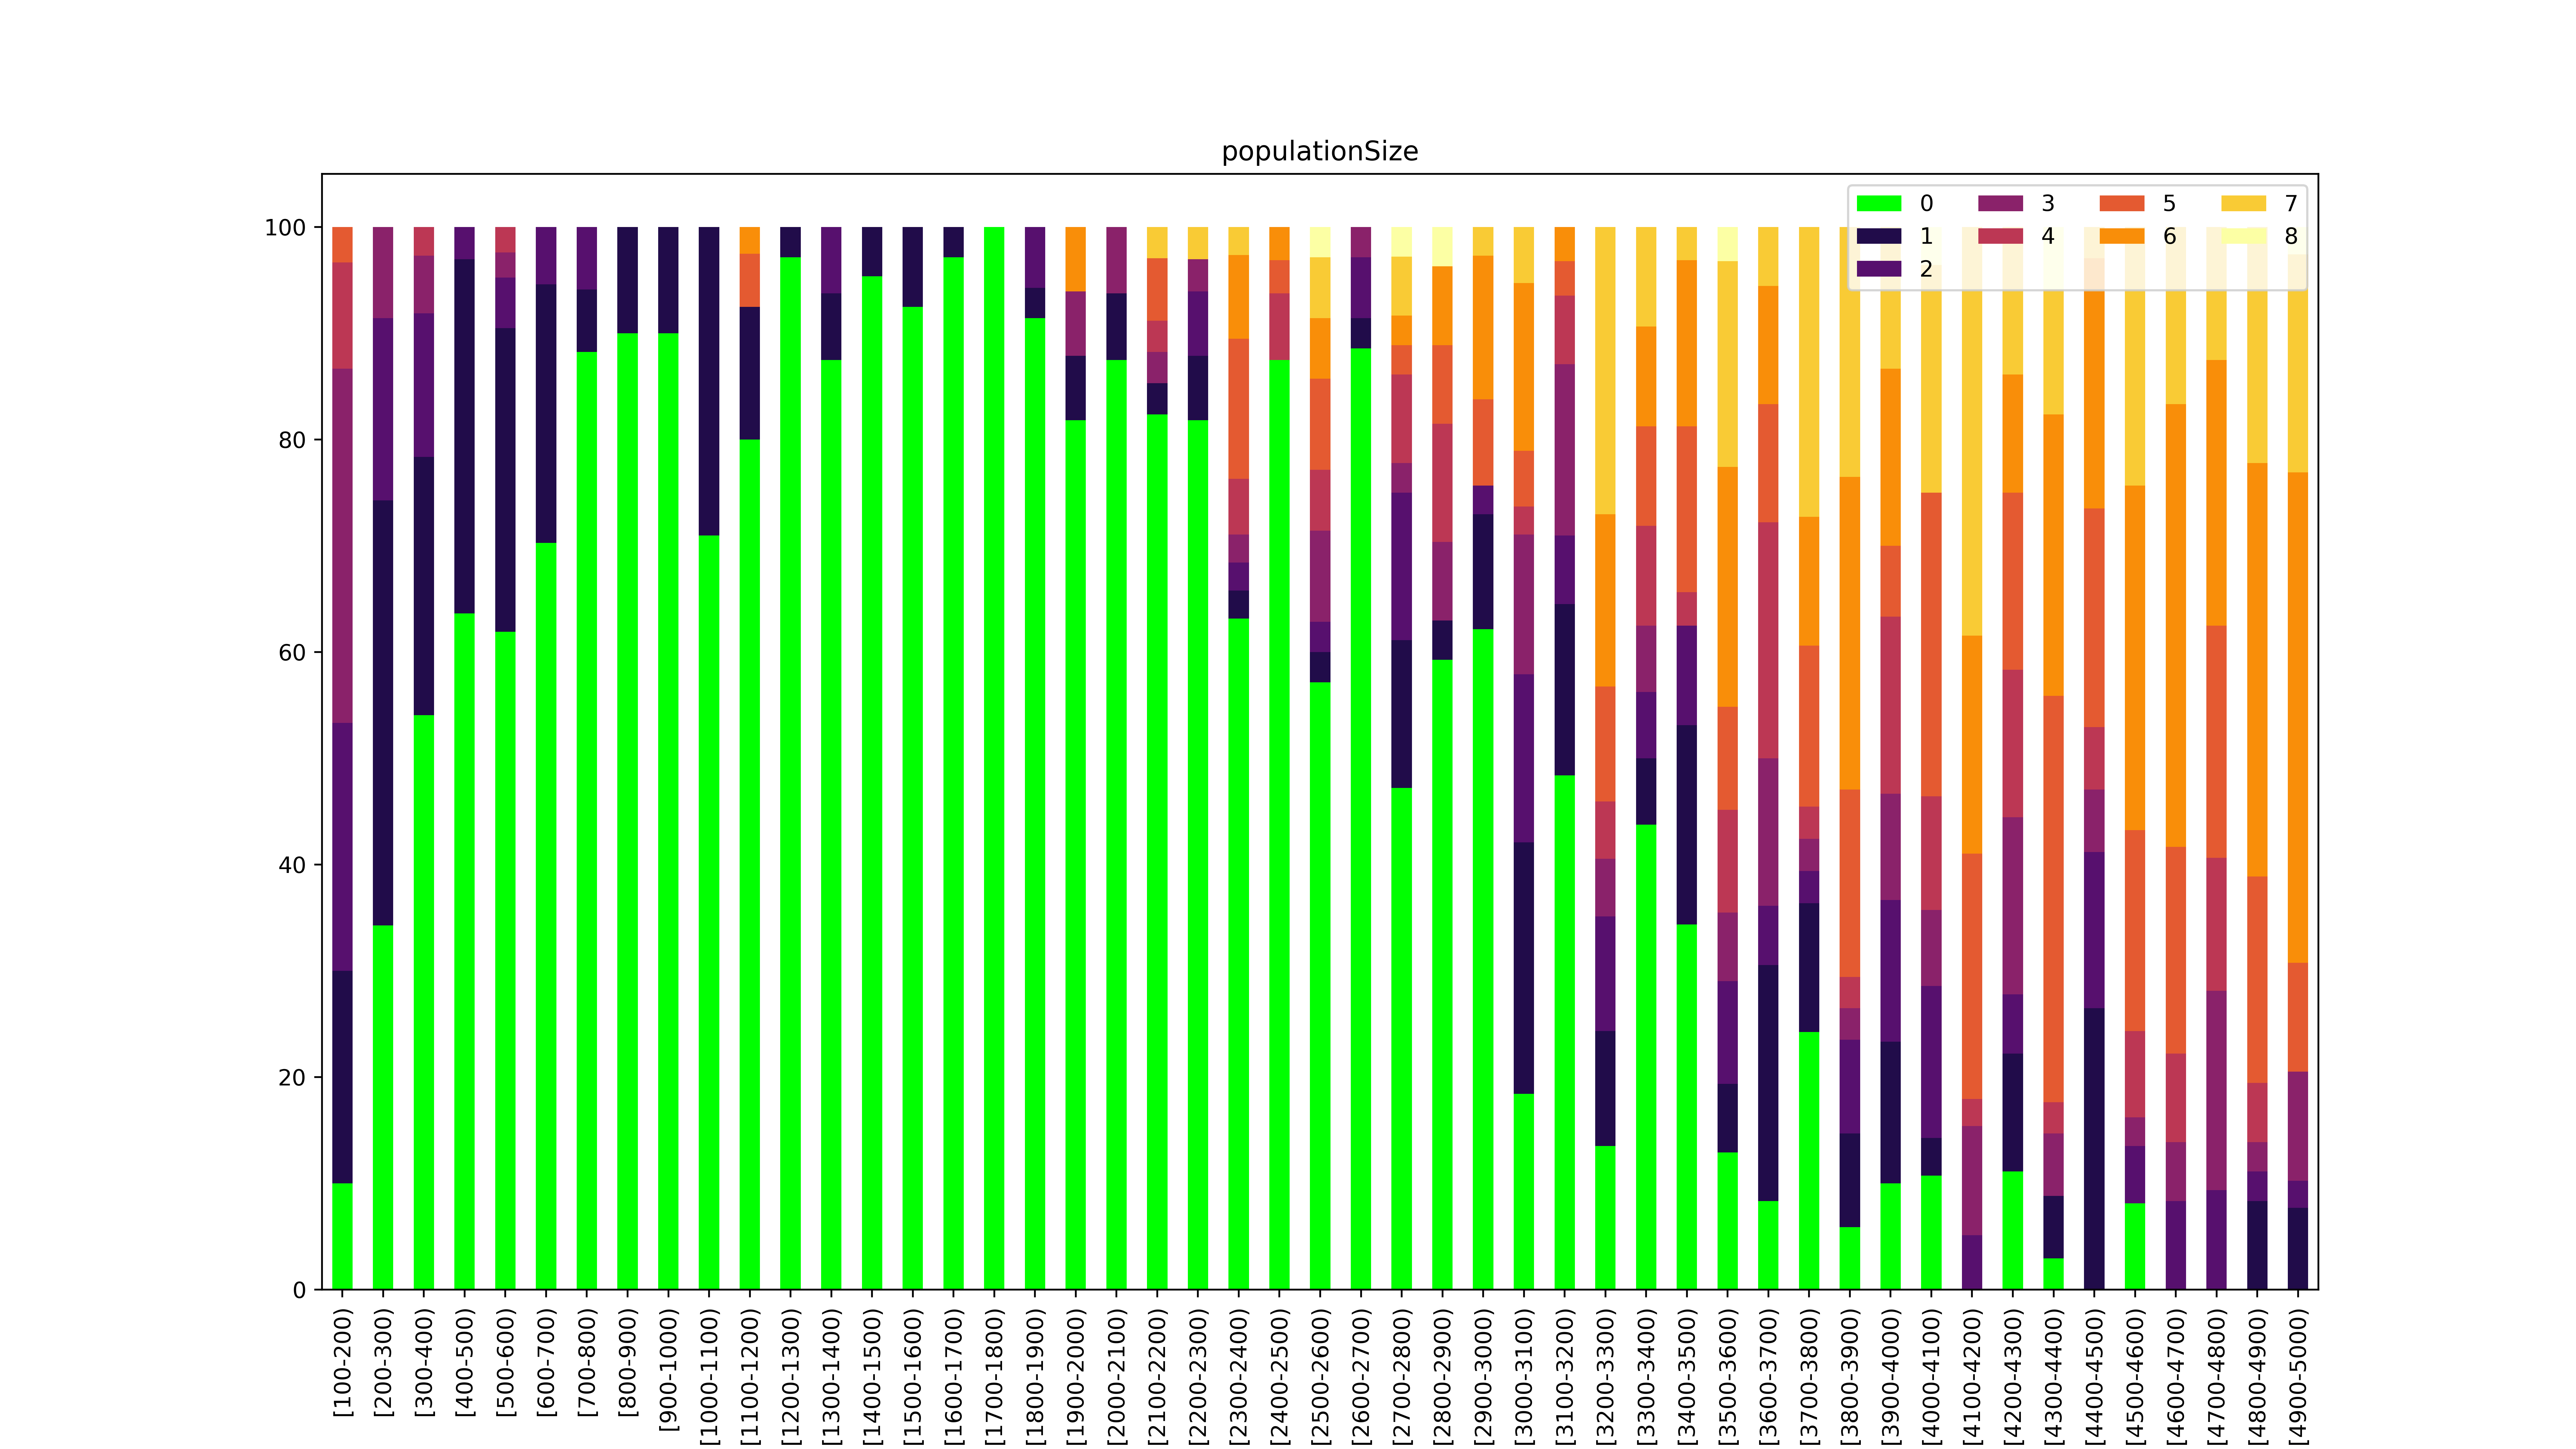
\includegraphics[clip,width=\textwidth]{images/populationSize_gradientSmall.png}%
	}
	
	\caption{main caption}	
\end{figure}

The next step in the analysis is the distribution of the parameter value and the number of contract violations that he gave. Consider the distribution of the population size parameter.
The color indicates the number of contract violations. The column height of a specific color is a percentage of the total number of configurations that have the same value. As can be seen, valid solutions are in the range from 1000 to 2600, which confirms the conclusion from the last step.

For a more visual image, we construct a similar graph for the smaller problem. This problem described with parameters: variants - 2, depth - 2, requests - 2, resources - 5.
It is shown in Figure~\ref{fig:populationSize_gradientSmall}. If we compare Figure~\ref{fig:populationSize_gradientSmall} and Figure~\ref{fig:populationSize_gradientBig}, we can see that they have a similar distribution.

\begin{figure}
	\centering
	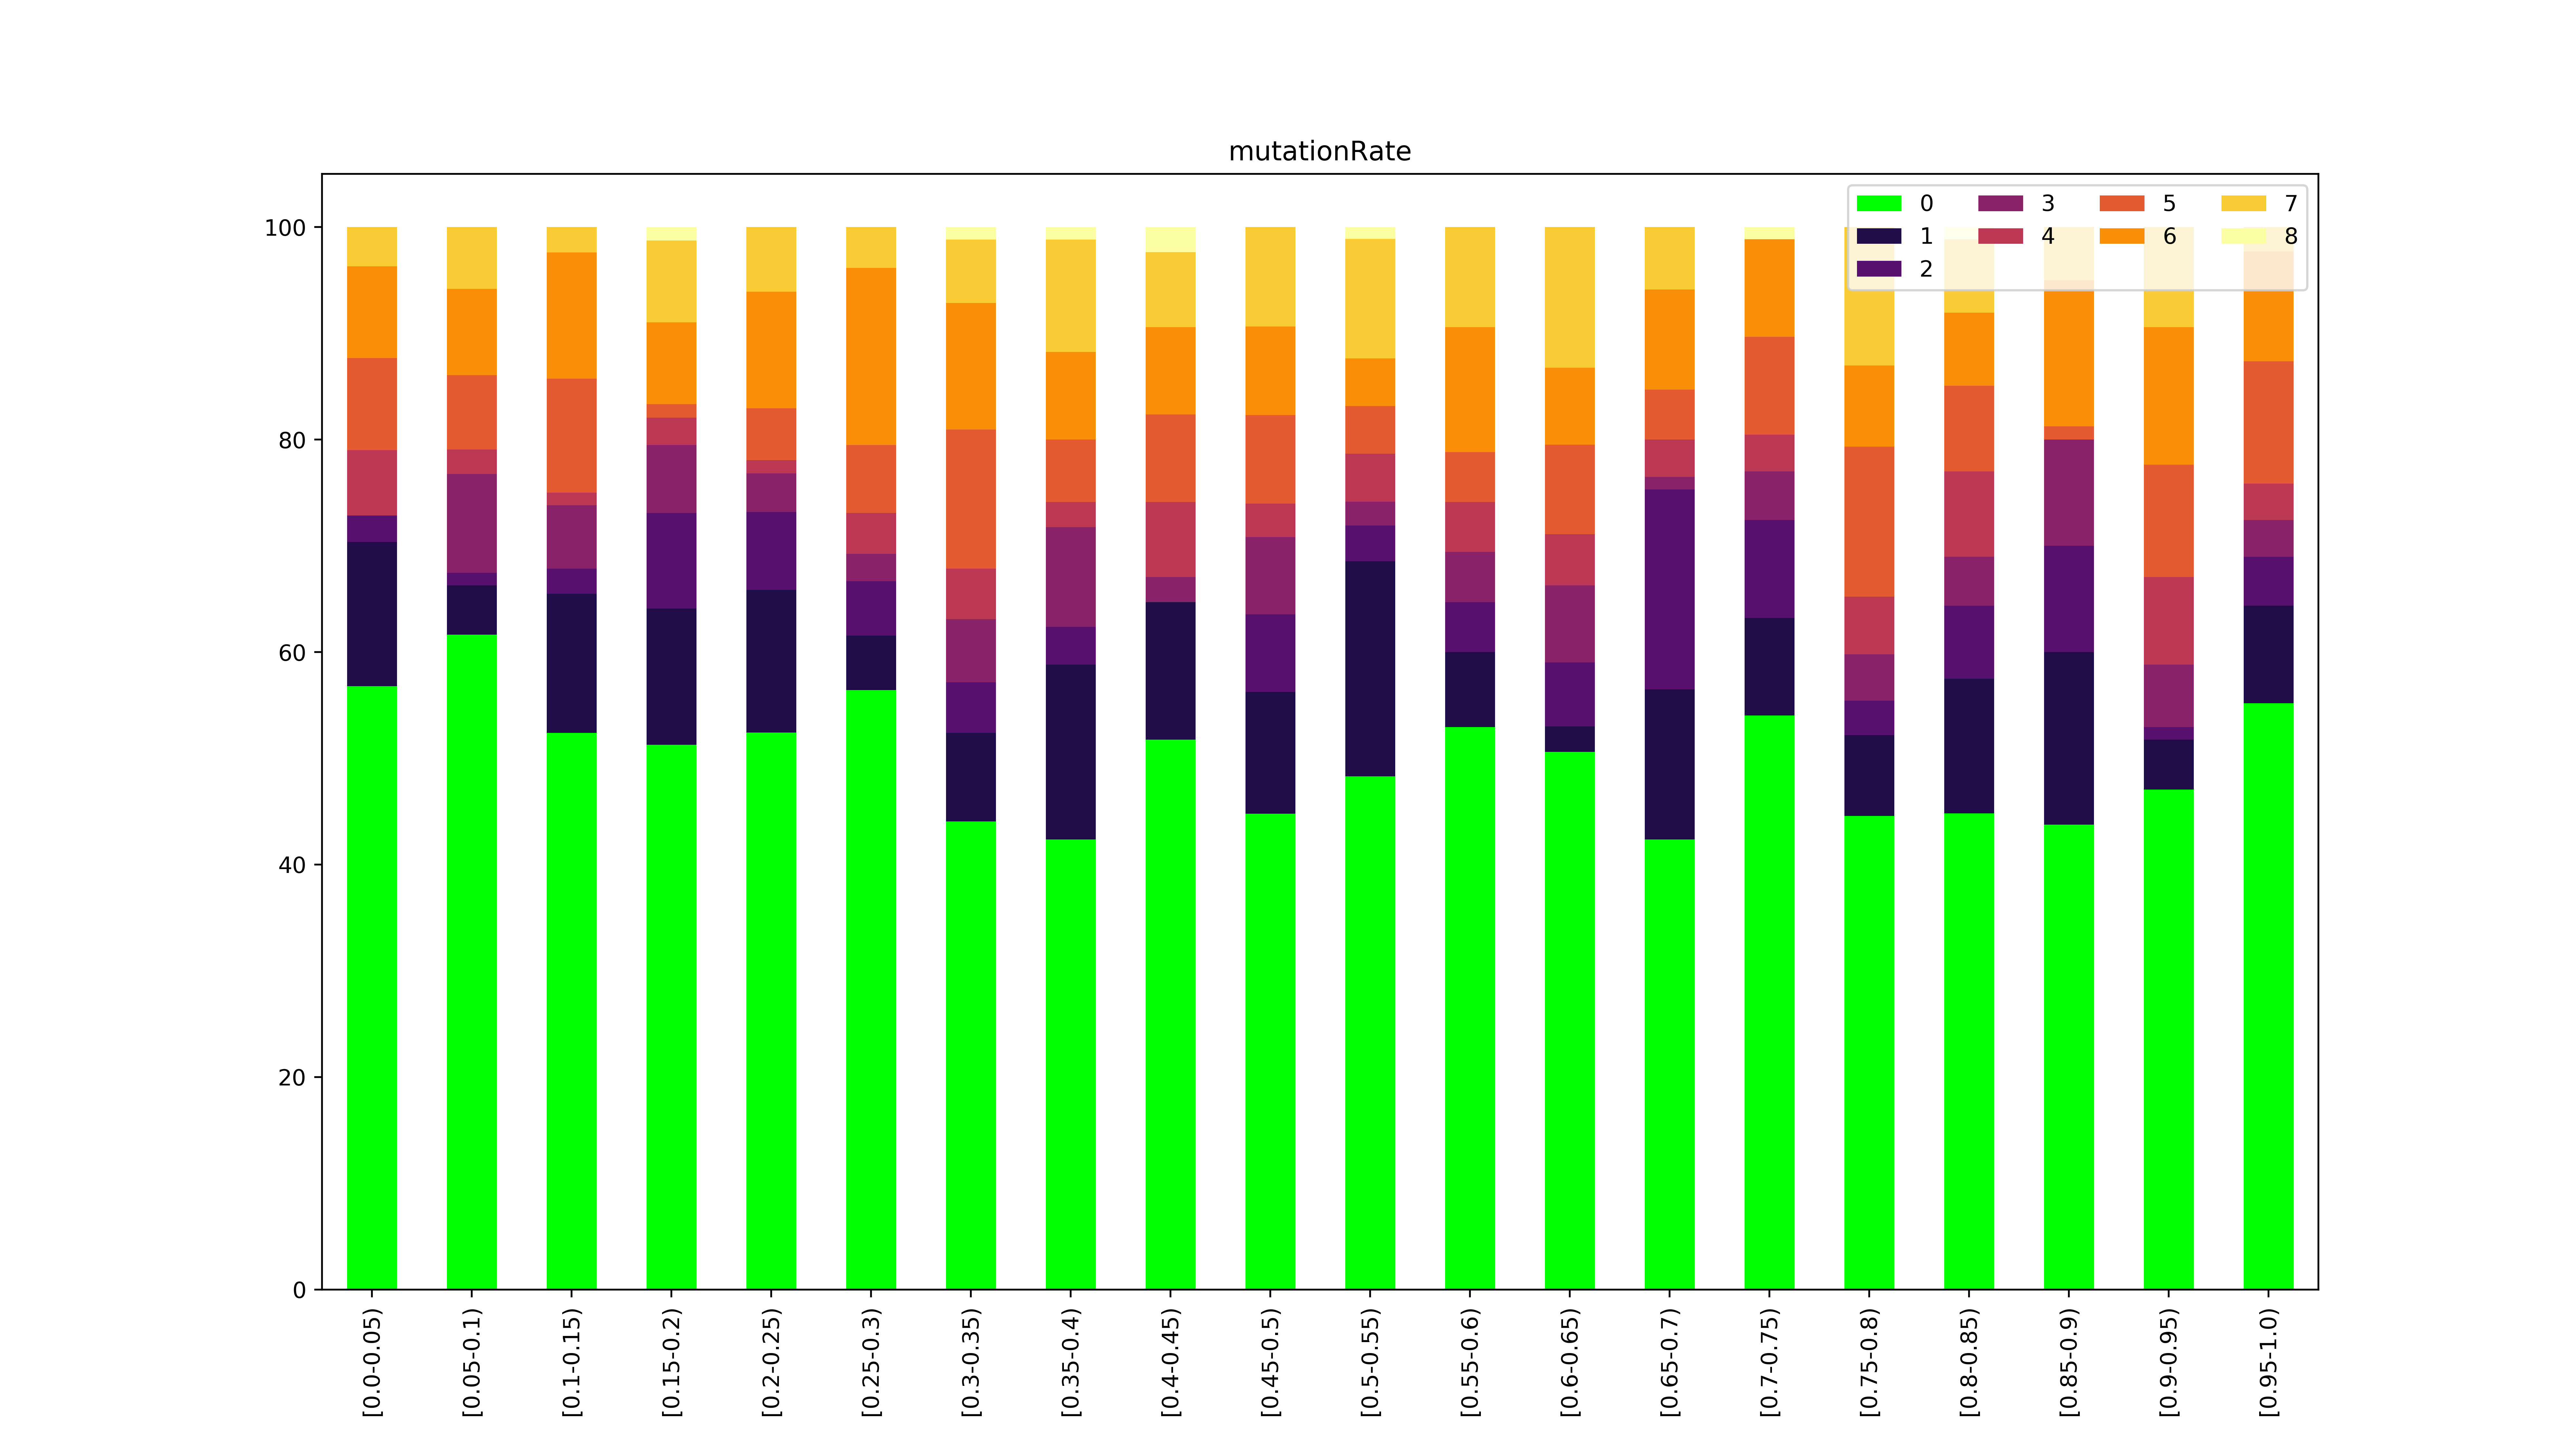
\includegraphics[width=\textwidth]{images/mutationRate_gradient_500dpi.png}
	\caption[]]{}
	\label{fig:mutationRate_gradient}
\end{figure}

The distributions of most parameters look like the distribution of the mutation rate parameter outlined in Figure~\ref{fig:mutationRate_gradient}.

Such a distribution means that the result of the solver does not matter from the value of the specific parameter.

\begin{figure}
	\centering
	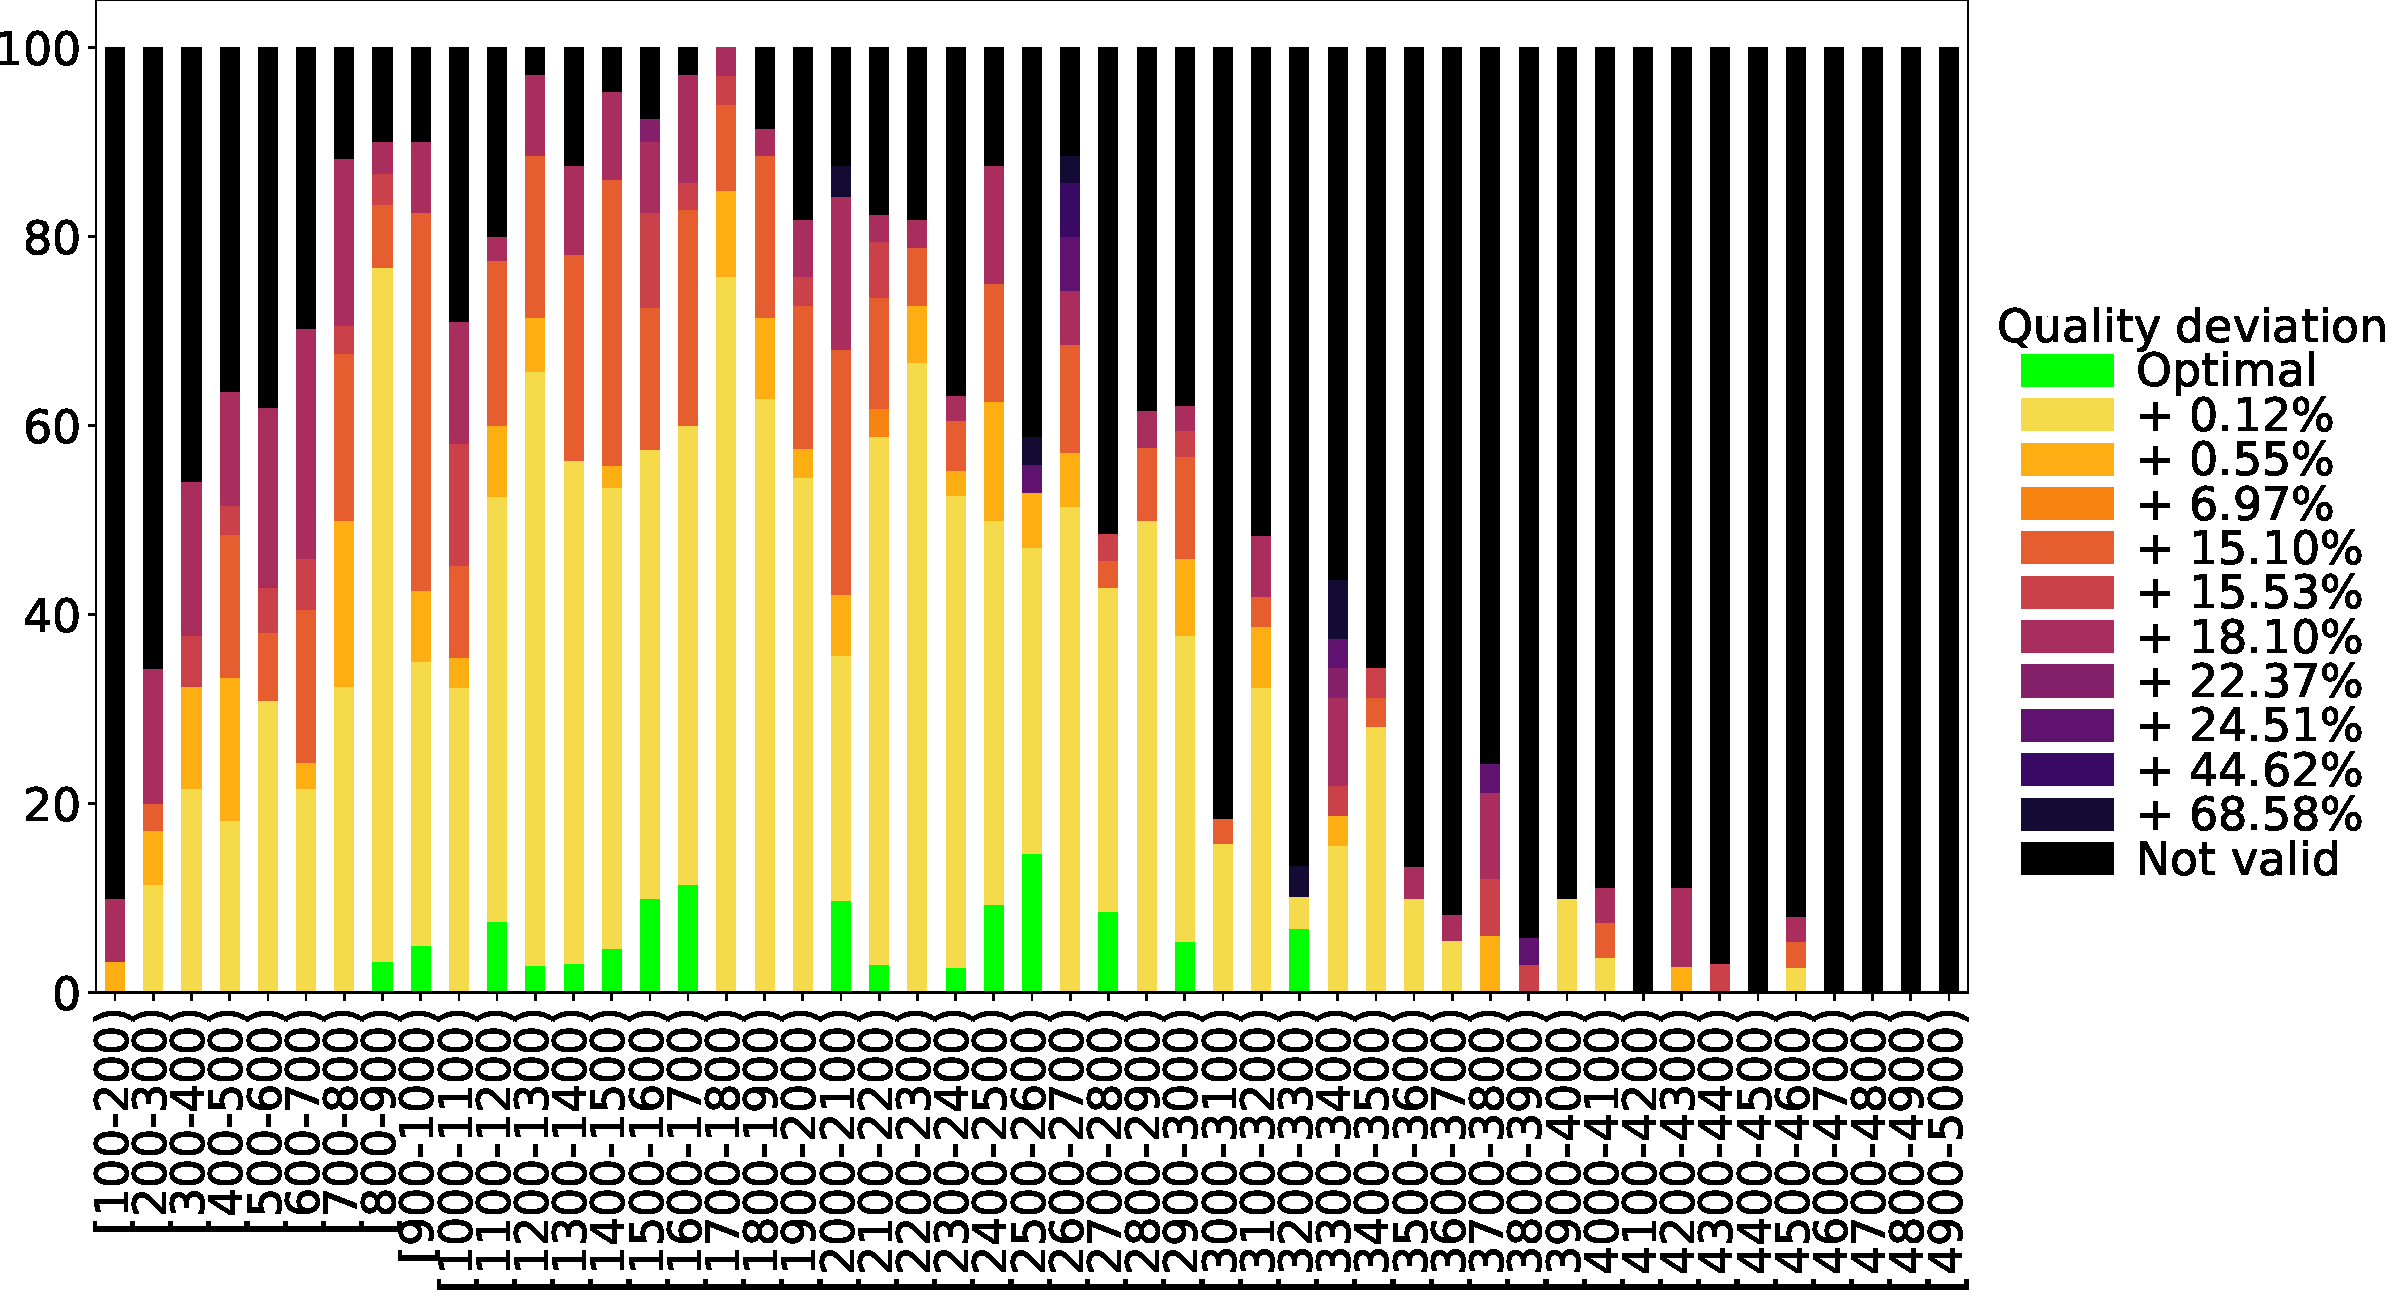
\includegraphics[width=\textwidth]{images/populationSizeObjective.pdf}
	\caption[]]{}
	\label{fig:populationSizeObjective}
\end{figure}

As for energy, let's build the distribution of the obtained energy values for the same parameters (Figure~\ref{fig:populationSizeObjective}).

This distribution proves the fact that if the solver found a valid solution, then this solution is optimal, or close to it.